\part{Etat de l'art} % (fold)
\label{prt:etat}
	\section{SSVEP} % (fold)
	SSVEP est l'abréviation de Steady State Visually Evoked Potential, traduit en français par l'état potentiel stable visuellement évoqué. Cela désigne, en neurologie, un ensemble de signaux représentant des réponses naturelles à des stimulus visuels à des fréquences spécifiques. La fréquence dépend de la puissance en Hz du stimulus visuel reçu par la rétine, celui-ci variant entre 3,5 et 75 Hz. La réponse se traduit par une activité électrique générée par le cerveau de même fréquence. Cette réponse est directe car elle se produit dés que le stimuli visuel est présenté.
		Cette technique est très utilisée en même temps que l'électroencéphalographie en ce qui concerne la vision. Elle est beaucoup appréciée pour son absence d'artefacts qui sont des effets artificiels parfois indésirables en plus du fait que les bruits alentours ne soient pas pris en compte.
	\label{sec:technique_ssvep}
	
	\section{P300} % (fold)
	Le P300 est un potentiel évoqué (modification du potentiel électrique produite par le système nerveux en réponse à une simulation externe (son, image, etc...) ou interne attention, préparation motrice, etc...), et plus généralement une onde positive et d'amplitude 300 ms. Cela signifie que la réponse n'est pas directe et qu'elle n'intervient que 300 ms après que la simulation ait eu lieu. Cette technique est notamment beaucoup utilisée dans l'électroencéphalographie.
			On distingue deux sous-types de P300 au sein de cette onde P300 aussi notée P3:
			\begin{itemize}
			\item[-] la P3a, généralement provoquée par un stimulus lors d'un effet de surprise;
			\item[-] la P3b où le sujet se trouve face à un stimulus non prévisible où il doit apporter une réponse (prise de décision, action réalisée grâce à la mémoire, etc...).
\end{itemize}			
	\label{sec:technique_p300}
	\section{BCI} % (fold)
				\begin{figure}[h]
		\centering 
	 	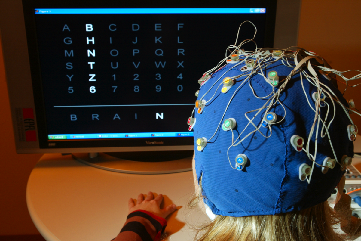
\includegraphics [width=7cm,height=7cm]{figures/bci3.png} \\
		\captionof{figure}{Photo d'un sujet en face d'une interface SSVEP}
		\label{fig_captors}	
	\end{figure}
		Ce procédé consiste en fait à restaurer, au moins partiellement des facultés perdues, voire non connues (dans le cas d'un handicap de naissance). C'est le cas notamment d'une personne ayant perdu totalement la vue à qui on a implanté un tel procédé au niveau de son cortex visuel, ce qui lui a permis de percevoir de nouveau la lumière. Si ces procédés ne sont pas miraculeux pour le moment, ils peuvent également permettre d'effectuer des actions par l'intermédiaire de la pensée. Ainsi, des personnes ont pu écrire sur un écran d'ordinateur ou déplacer le curseur d'une souris en imaginant simplement l'action de le faire. D'autres ont pu déplacer un bras robotisé pour qu'il leur ramène quelque chose par exemple.

	Ce procédé peut être unidirectionnel (la machine envoie des données au cerveau ou le contraire mais pas les deux en même temps) ou bidirectionnel.
	Ces interfaces neuronales directes présentent toutefois plusieurs limites:
	\begin{itemize}
		\item [-] chacune d'elles ne fait qu'une tâche précise et non plusieurs;
		\item [-] elles étaient initialement développées dans un but médical rendant l'accès difficile au grand public;
		\item [-] à cela s'ajoute le fait que les populations défavorisées n'auront pas les moyens de se procurer de tels équipements, le prix étant très élevé.
	\end{itemize}
	\label{sec:bci}
	\section{Applications Médicales} % (fold)
		Les applications du programme que nous développons peut servir pour des études très variées sur plusieurs types de pathologies telles que la maladie d'Alzheimer ou encore les crises d'épilepsies que l'on peut prévoir et minimiser notamment, pour ne citer que ces deux exemples. On peut aussi l'utiliser comme moyen ludique pour détecter la concentration des élèves en classe en temps réel. On pourrait aussi, à l'avenir, contrôler notre PC à l'aide de notre seule pensée au moyen d'un casque EEG.
	\label{sec:application_médical}
	
				
	
	% section application_médical (end)
	
	% section bci (end) 
	
	% section technique_p300 (end)  	
	
	% section technique_ssvep (end)
% part e_\_ (end)